\documentclass[final,t]{beamer}
\catcode`\@=11
\mode<presentation>
{
%  \usetheme{Warsaw}
%  \usetheme{Aachen}
%  \usetheme{Oldi6}
%  \usetheme{I6td}
  \usetheme{I6dv}
%  \usetheme{I6pd}
%  \usetheme{I6pd2}
}



\def\bold#1{\mbox {\bf #1}}\def \vc #1#2{\bold {#1}_{#2}}\def \bftil #1#2{\bold {\widetild #1}_{#2}}
\def\bea{ \begin{eqnarray}}
\def\eea{\end{eqnarray}}
\def\cref#1{(\ref {#1})}
\def\Let@{\relax\iffalse{\fi\let\\=\cr\iffalse}\fi}
\def\vspace@{\def\vspace##1{\noalign{\vskip##1 }}}
\def\mat{\left[\matrix} \def\endmat{\endmatrix\right]}
%\def\vspace@{\def\vspace##1{\noalign{\vskip##1 }}}
\def\matrix{\,\vcenter\bgroup\Let@\vspace@
    \normalbaselines
  \m@th\ialign\bgroup\hfil$##$\hfil&&\quad\hfil$##$\hfil\crcr
    \mathstrut\crcr\noalign{\kern-\baselineskip}}
\def\endmatrix{\crcr\mathstrut\crcr\noalign{\kern-\baselineskip}\egroup
\egroup\,}


% additional settings
\setbeamerfont{itemize}{size=\normalsize}
\setbeamerfont{itemize/enumerate body}{size=\normalsize}
\setbeamerfont{itemize/enumerate subbody}{size=\normalsize}

% additional packages
\usepackage{times}
\usepackage{amsmath,amsthm, amssymb, latexsym,epsfig}
\usepackage{exscale}
%\boldmath
\usepackage{booktabs, array}
%\usepackage{rotating} %sideways environment
\usepackage[brazil]{babel}
\usepackage[utf8]{inputenc}
\usepackage{natbib}
\usepackage{ragged2e}

\usepackage{subfigure}
\usepackage[orientation=landscape,size=custom,width=90,height=120,scale=1.15]{beamerposter}

\listfiles
\graphicspath{{figures/}}
% Display a grid to help align images
%\beamertemplategridbackground[1cm]



\title{\huge One century of data from Vassouras Magnetic Observatory (1915-2015).}


\author[Benevides, Bassrei]{Artur Benevides, Edwin Camacho*, Vitor Silveira, Israelli Rodrigo, Rodrigo Melhorato e Kátia Pinheiro}
\institute[ON-MCTIC]{Observatório Nacional}
\date[Nov , 2017]{Nov. 15 , 2017}


% abbreviations
\usepackage{xspace}
\makeatletter
\DeclareRobustCommand\onedot{\futurelet\@let@token\@onedot}
\def\@onedot{\ifx\@let@token.\else.\null\fi\xspace}
\def\eg{{e.g}\onedot} \def\Eg{{E.g}\onedot}
\def\ie{{i.e}\onedot} \def\Ie{{I.e}\onedot}
\def\cf{{c.f}\onedot} \def\Cf{{C.f}\onedot}
\def\etc{{etc}\onedot}
\def\vs{{vs}\onedot}
\def\wrt{w.r.t\onedot}
\def\dof{d.o.f\onedot}
\def\etal{{et al}\onedot}
\makeatother

%%%%%%%%%%%%%%%%%%%%%%%%%%%%%%%%%%%%%%%%%%%%%%%%%%%%%%%%%%%%%%%%%%%%%%%%%%%%%%%%%%%%%%%%%%%%%%%%%%%%%%%%%%%%
%%%%%%%%%%%%%%%%%%%%%%%%%%%%%%%%%%%%%%%%%%%%%%%%%%%%%%%%%%%%%%%%%%%%%%%%%%%%%%%%%%%%%%%%%%%%%%%%%%%%%%%%%%%%
\begin{document}

  \begin{columns}[t]
    \begin{column}{.33\linewidth}

%%%%%%%%%%%%%%%%%%%%%%%%%%%%%%%%%%%%%%%%%%%%%%%%%%%%%%%%%%%%%%%%%%%%%%%%%%%%%%%%%%%%%%%%%%%%%%%%%%%%%%%%%%%%
%%%%%%%%%%%%%%%%%%%%%%%%%%%%%%%%%% Primeira coluna %%%%%%%%%%%%%%%%%%%%%%%%%%%%%%%%%%%%%%%%%%%%%%%%%%%%%%%%%
%%%%%%%%%%%%%%%%%%%%%%%%%%%%%%%%%%%%%%%%%%%%%%%%%%%%%%%%%%%%%%%%%%%%%%%%%%%%%%%%%%%%%%%%%%%%%%%%%%%%%%%%%%%%
\begin{block}{Introdução}
	
\begin{itemize}
\justifying
		\item Vassouras Magnetic Observatory (VSS) was the first observatory in Brazil, starting its	measurements in 1915. VSS is part of the INTERMAGNET since 1998 because of its high data quality and transmission in real time. The centennial observations of magnetic field components in Vassouras are fundamental to global models, especially because of the lack of data in the Southern Hemisphere. Global models contribute significantly on the understanding of the Earth's magnetic field, both internal field caused by core dynamics, and external source, produced in the ionosphere and magnetosphere. Data from VSS is also applied to studies on geophysical prospection of metals and hydrocarbons.
		
		\item This work presents the history of VSS as well as the centennial dataset (1915-2015). We	explore the comparison of VSS data and results of IGRF model
		
		\item  Presentation of Sq and storm data and comparison with CHAOS model
		
		\item The main characteristics of the secular variation in
		VSS
		
		\item The possible geomagnetic jerks occurring in this period.	
		
	\end{itemize}
	
\end{block}

\begin{block}{Geomagnetic field (1915-2015)}

\begin{figure}
	\centering
	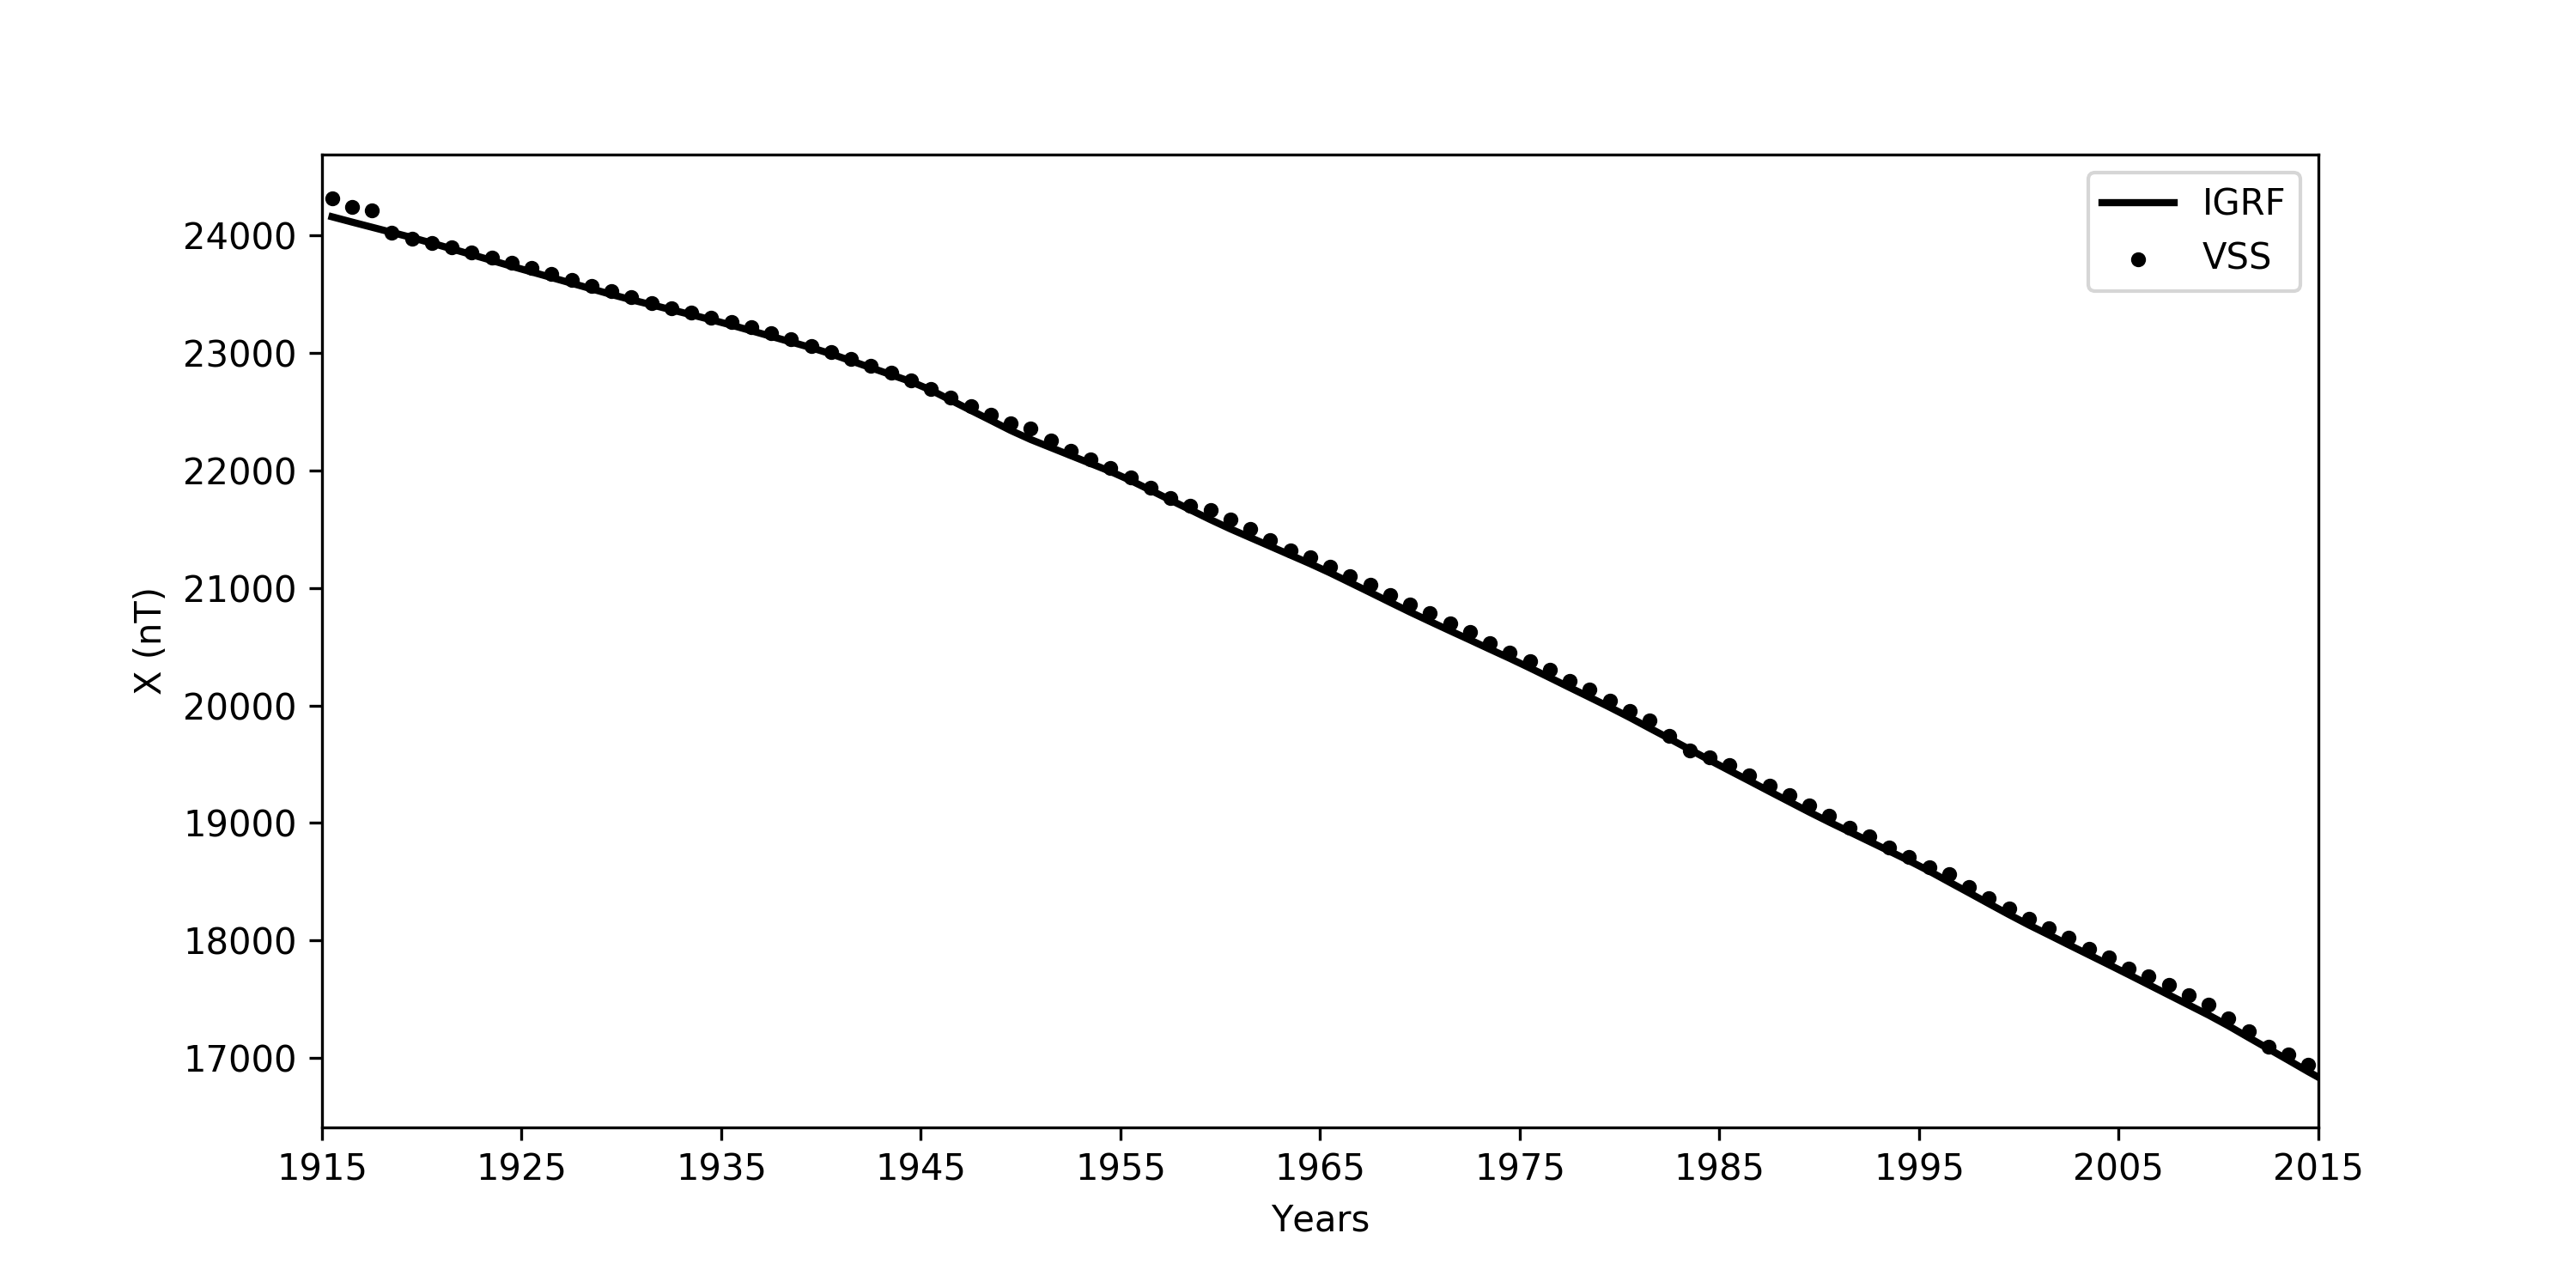
\includegraphics[width=1.0\linewidth]{X}
	\caption{2. Resultados das inversões SVD pra os modelos sintéticos I e II.}
	\label{fig:g_Sintetico}
\end{figure}

\begin{figure}
	\centering
	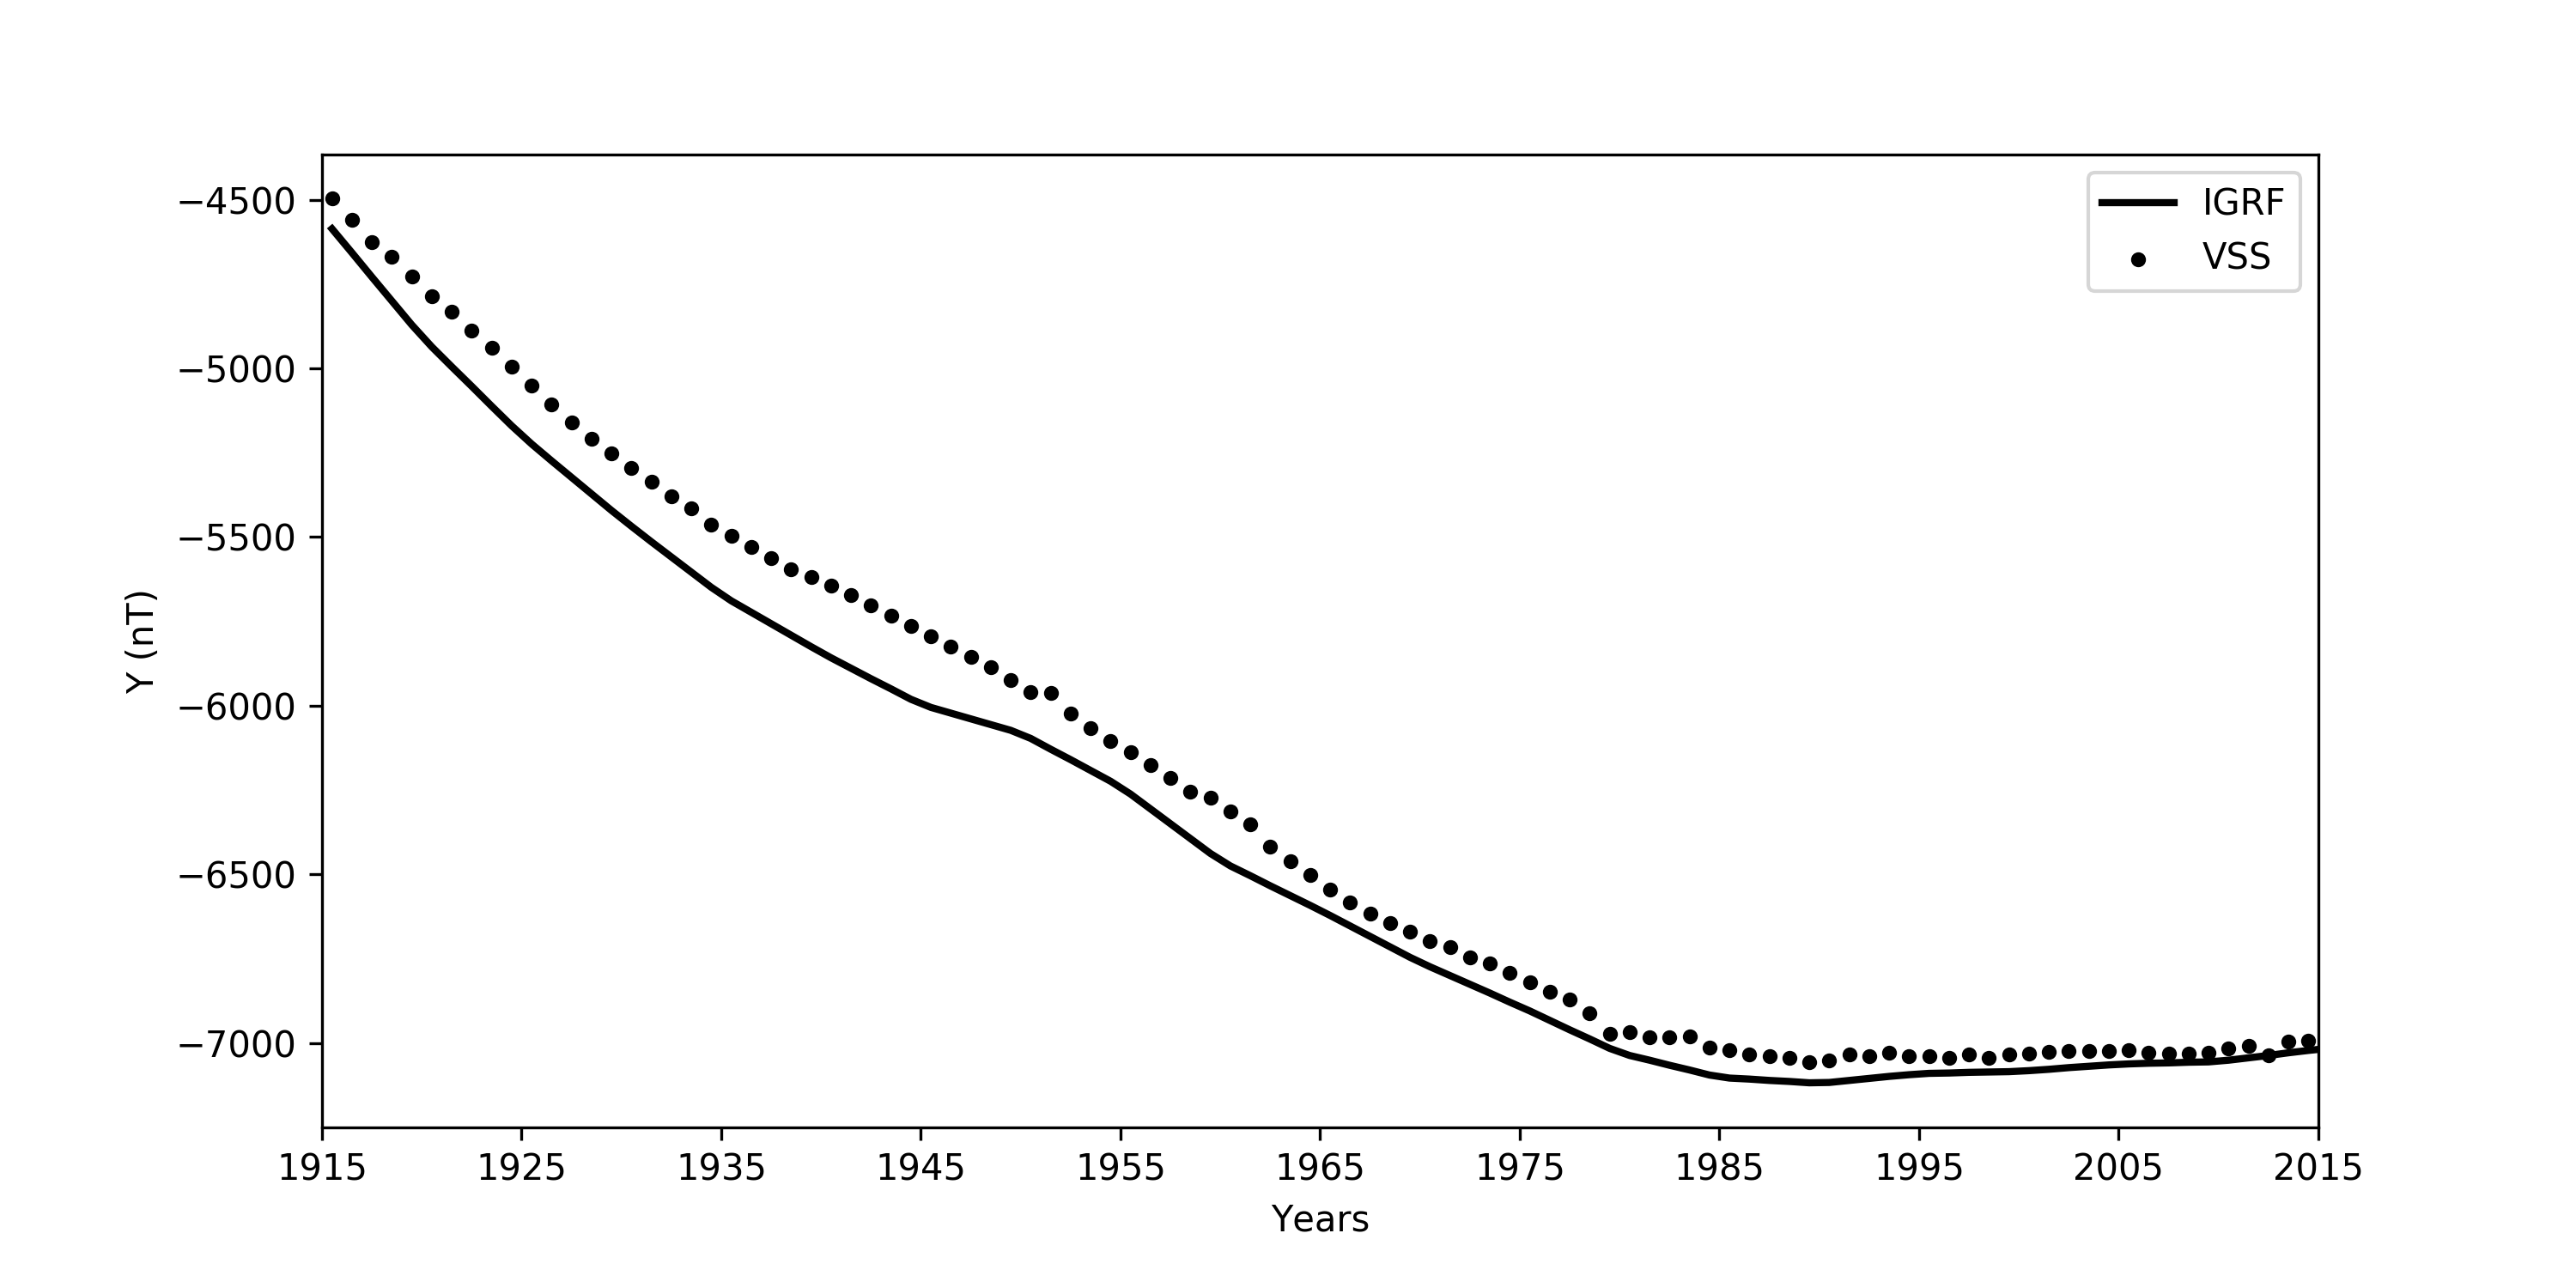
\includegraphics[width=1.0\linewidth]{Y}
	\caption{2. Resultados das inversões SVD pra os modelos sintéticos I e II.}
	\label{fig:g_Sintetico}
\end{figure}

\begin{figure}
	\centering
	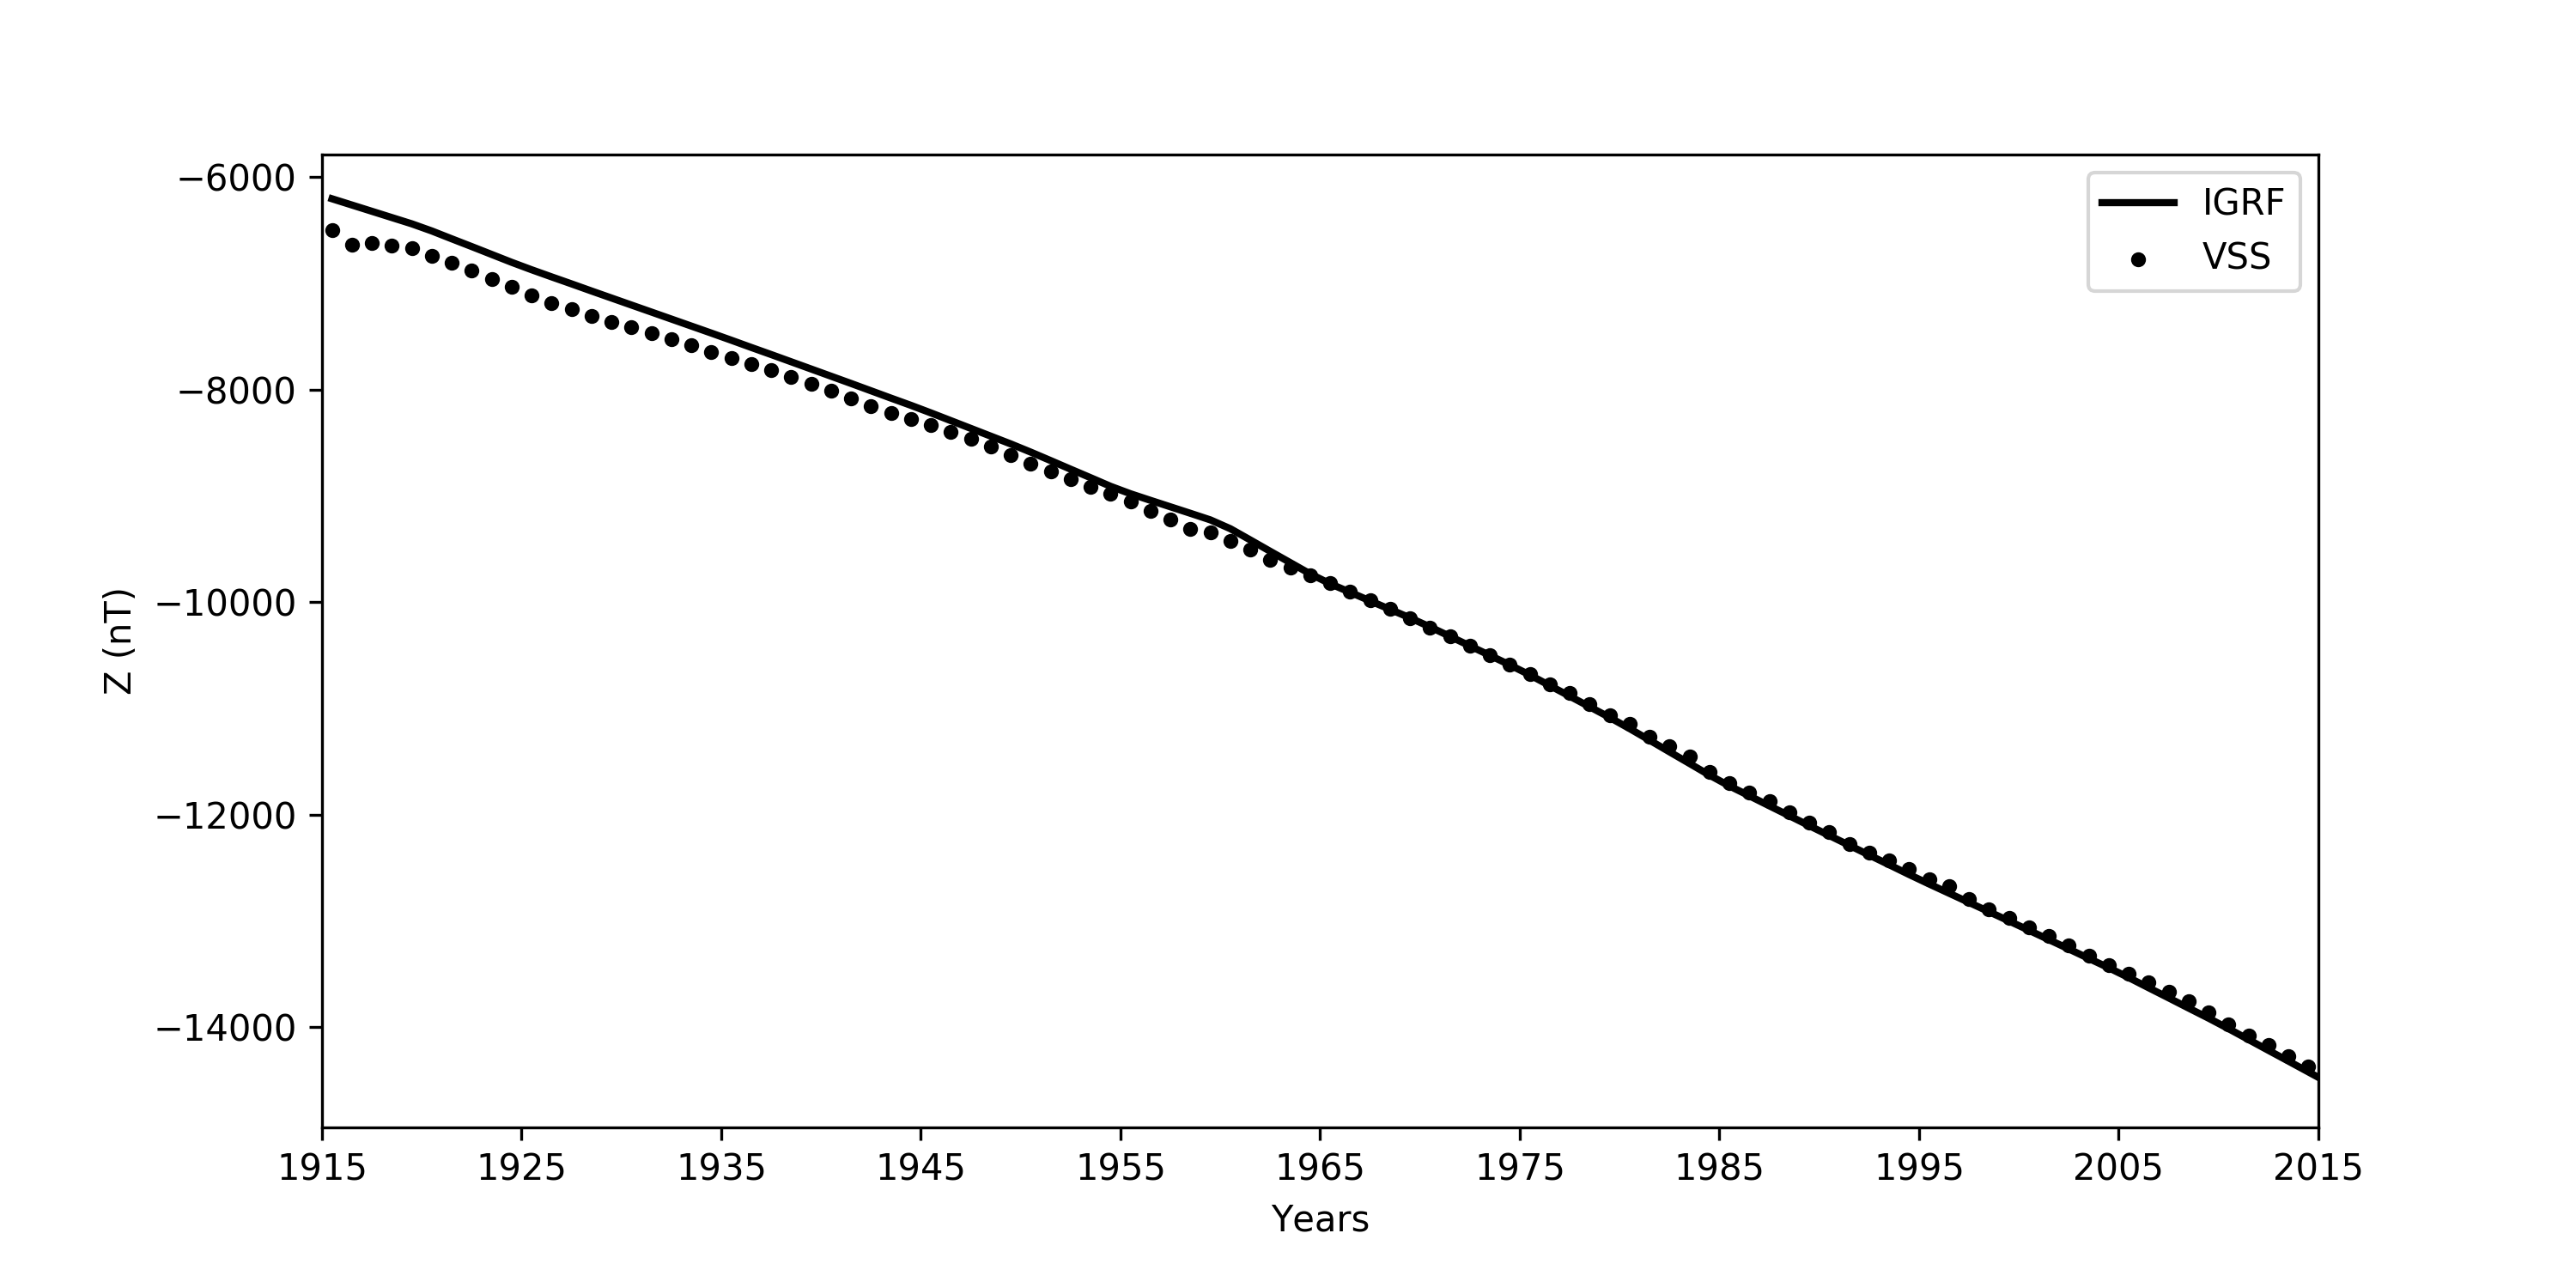
\includegraphics[width=1.0\linewidth]{Z}
	\caption{2. Resultados das inversões SVD pra os modelos sintéticos I e II.}
	\label{fig:g_Sintetico}
\end{figure}

\begin{figure}
	\centering
	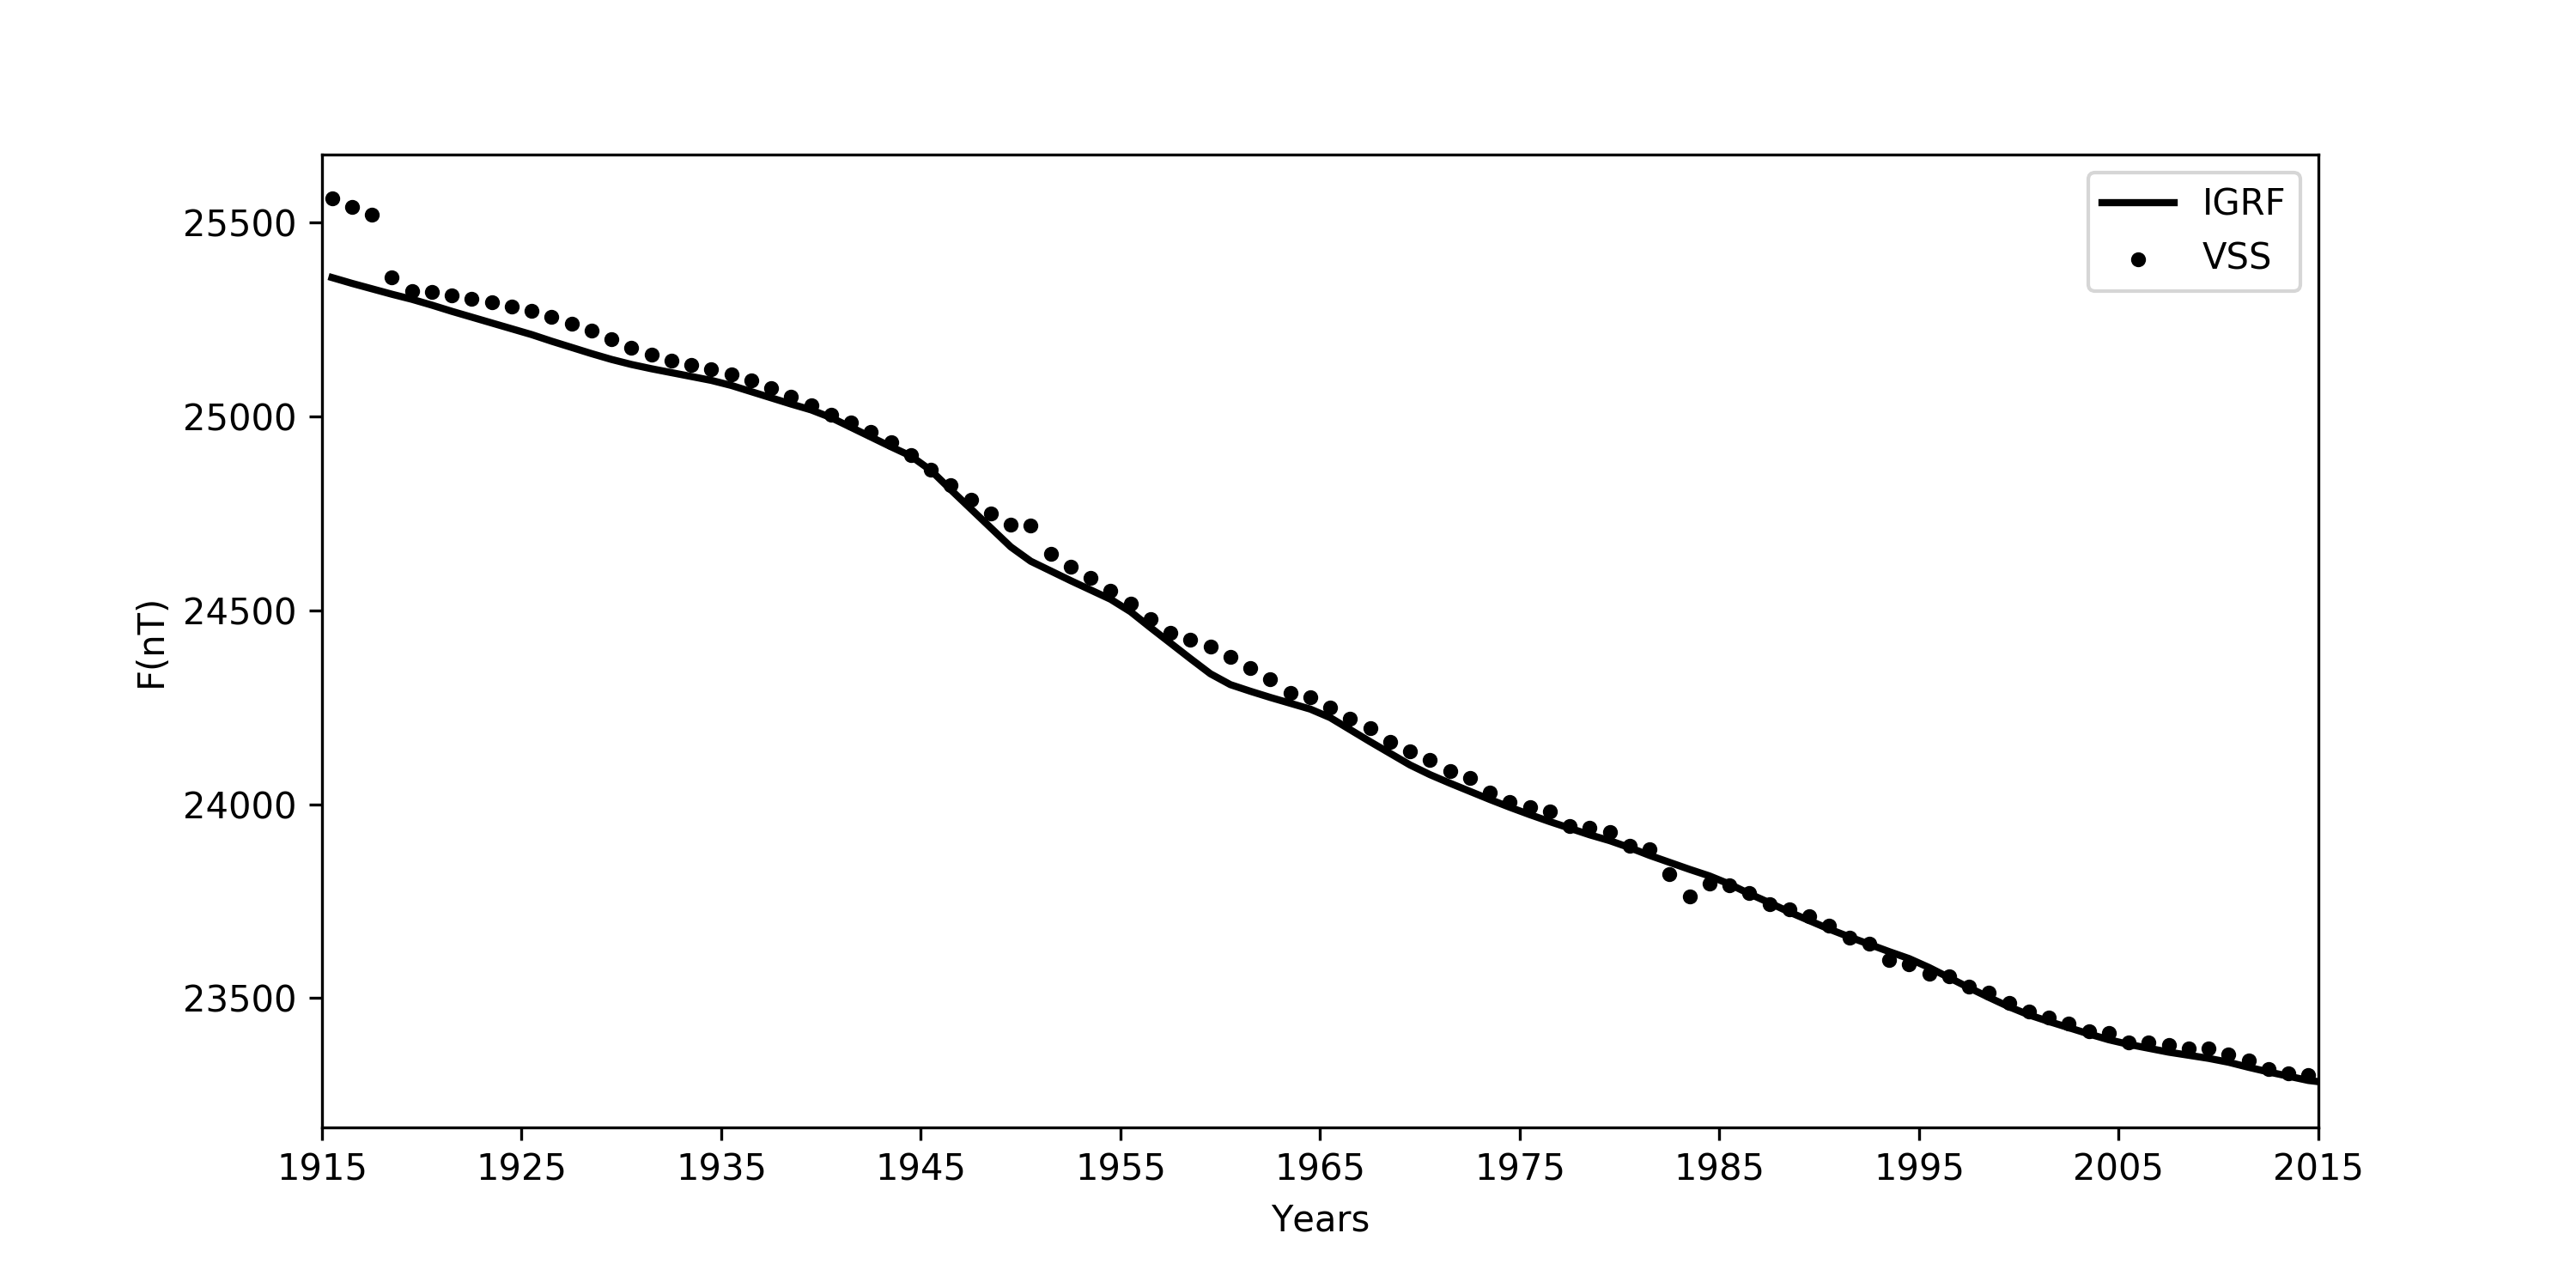
\includegraphics[width=1.0\linewidth]{F}
	\caption{2. Resultados das inversões SVD pra os modelos sintéticos I e II.}
	\label{fig:g_Sintetico}
\end{figure}

\end{block}	


\end{column}
%%%%%%%%%%%%%%%%%%%%%%%%%%%%%%%%%%%%%%%%%%%%%%%%%%%%%%%%%%%%%%%%%%%%%%%%%%%%%%%%%%%%%%%%%%%%%%%%%%%%%%%%%%%%%%%%%%%%%%%%%%%%
%%%%%%%%%%%%%%%%%%%%%%%%%%%%%%%%%%%%%%%%%%%%%%%%%%% Segunda coluna %%%%%%%%%%%%%%%%%%%%%%%%%%%%%%%%%%%%%%%%%%%%%%%%%%%%%%%%%
%%%%%%%%%%%%%%%%%%%%%%%%%%%%%%%%%%%%%%%%%%%%%%%%%%%%%%%%%%%%%%%%%%%%%%%%%%%%%%%%%%%%%%%%%%%%%%%%%%%%%%%%%%%%%%%%%%%%%%%%%%%%
\begin{column}{.31\linewidth}

\begin{block}{}
	\justifying
	

	\begin{figure}
		\centering
		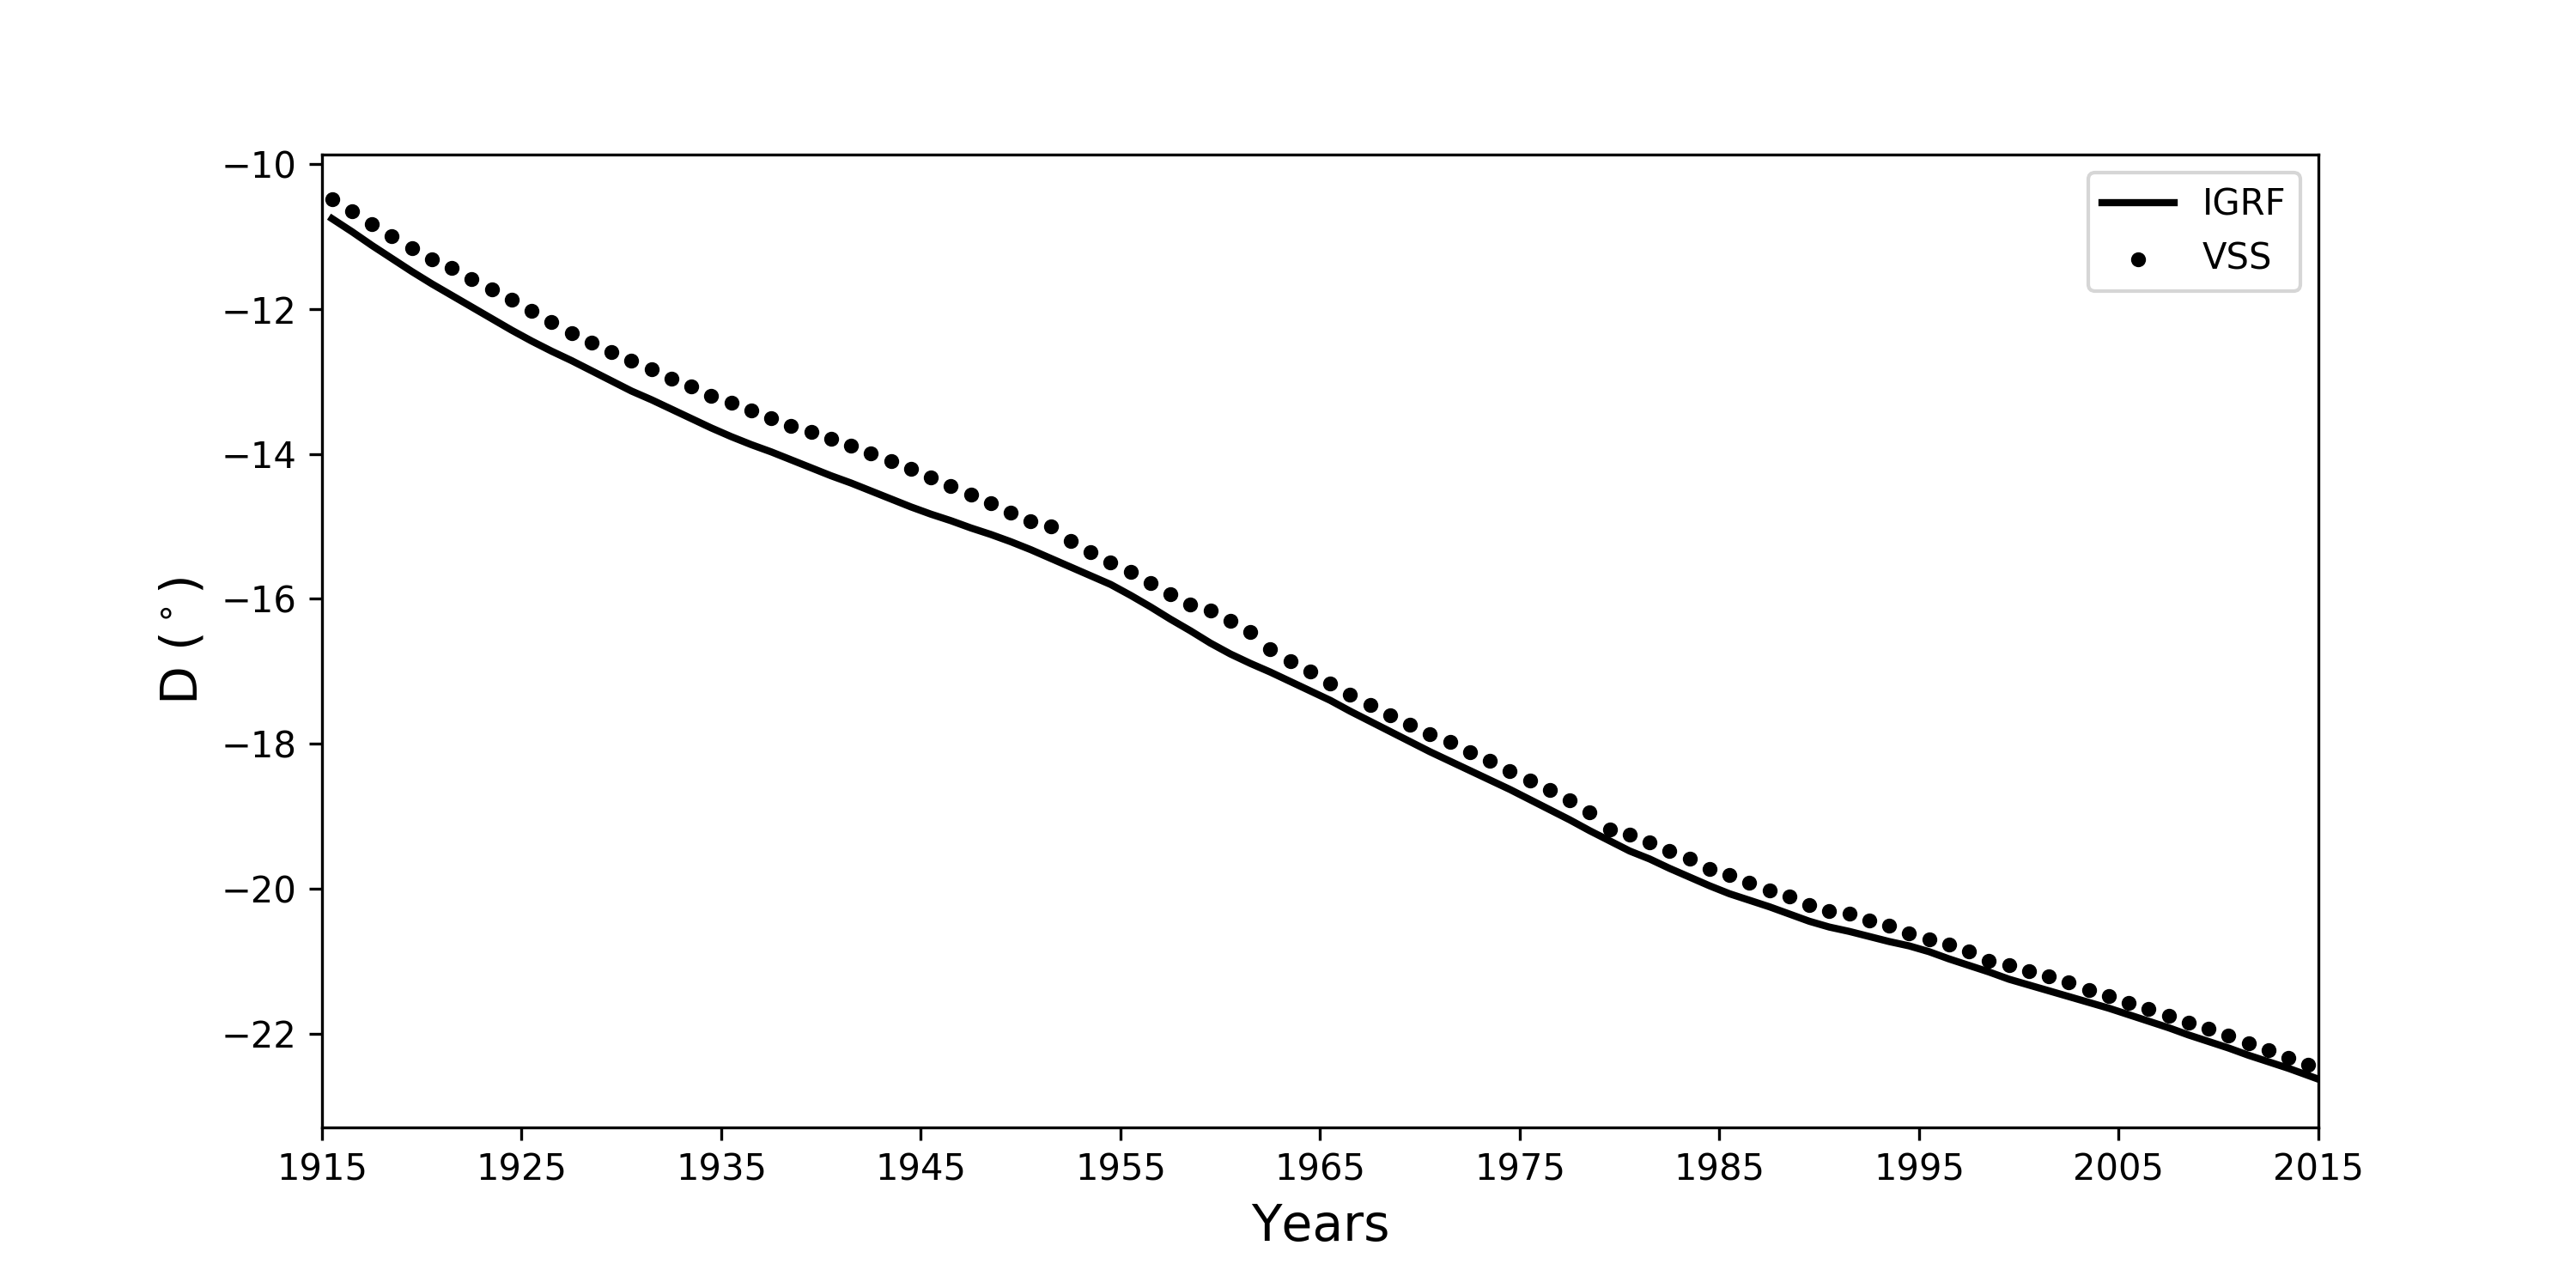
\includegraphics[width=1.0\linewidth]{D}
		\caption{2. Resultados das inversões SVD pra os modelos sintéticos I e II.}
		\label{fig:g_Sintetico}
	\end{figure}
	
		
		\begin{figure}
			\centering
			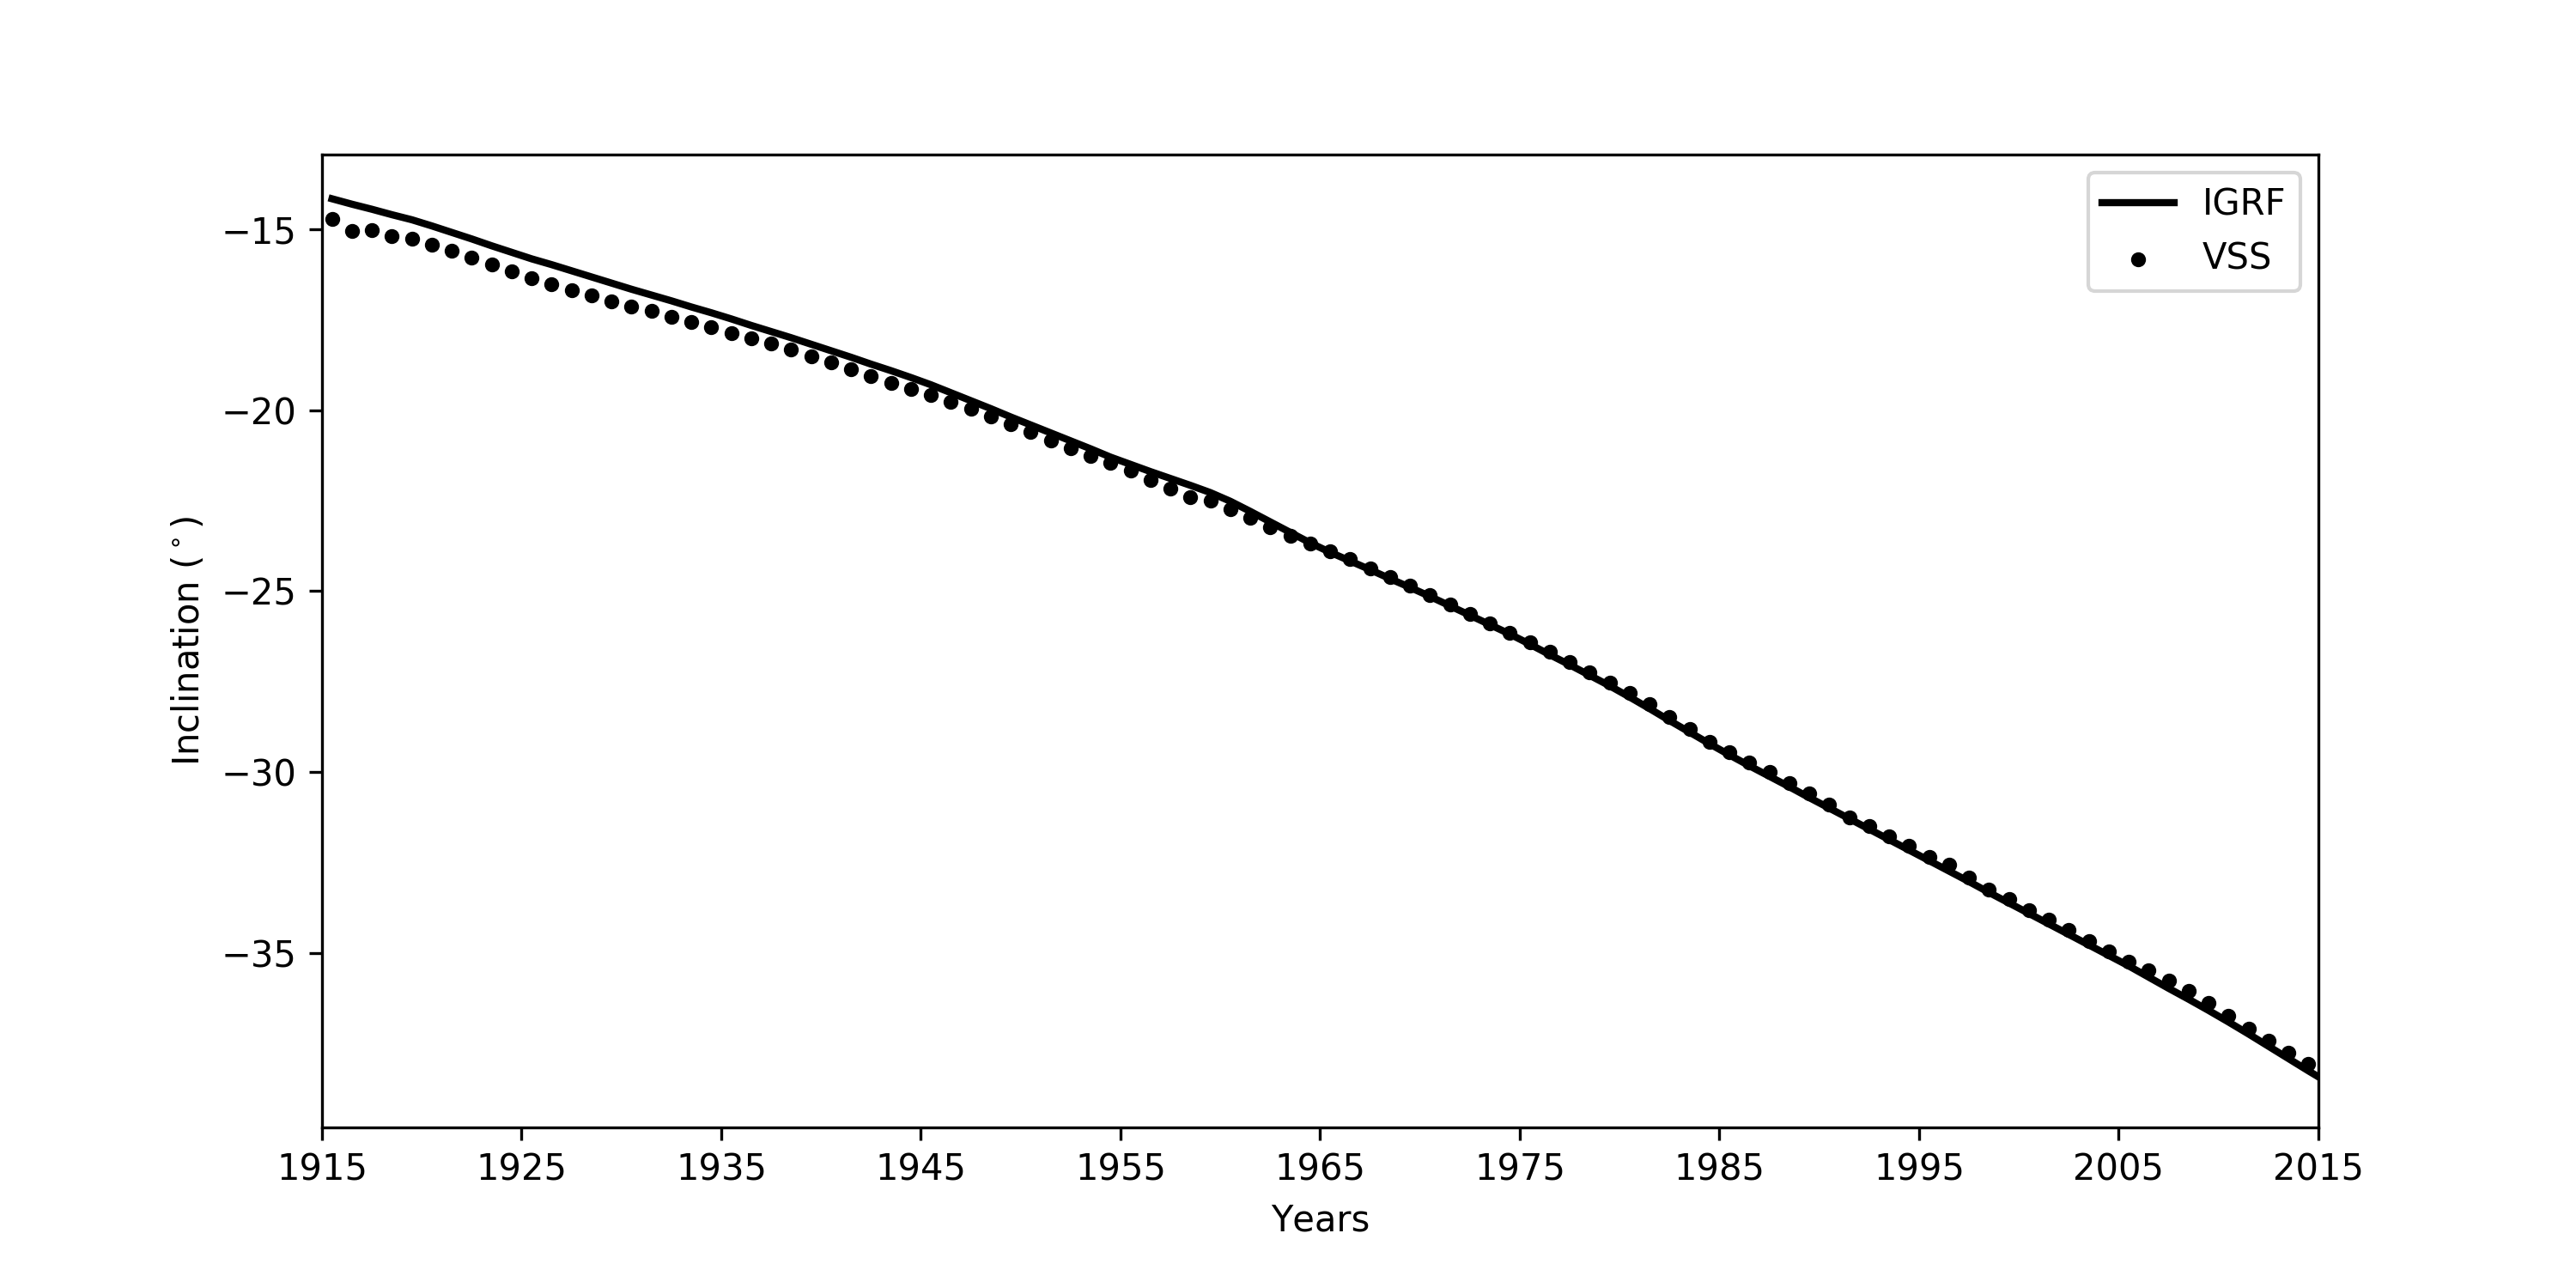
\includegraphics[width=1.0\linewidth]{I}
			\caption{2. Resultados das inversões SVD pra os modelos sintéticos I e II.}
			\label{fig:g_Sintetico}
		\end{figure}
	
	
		\begin{figure}
			\centering
			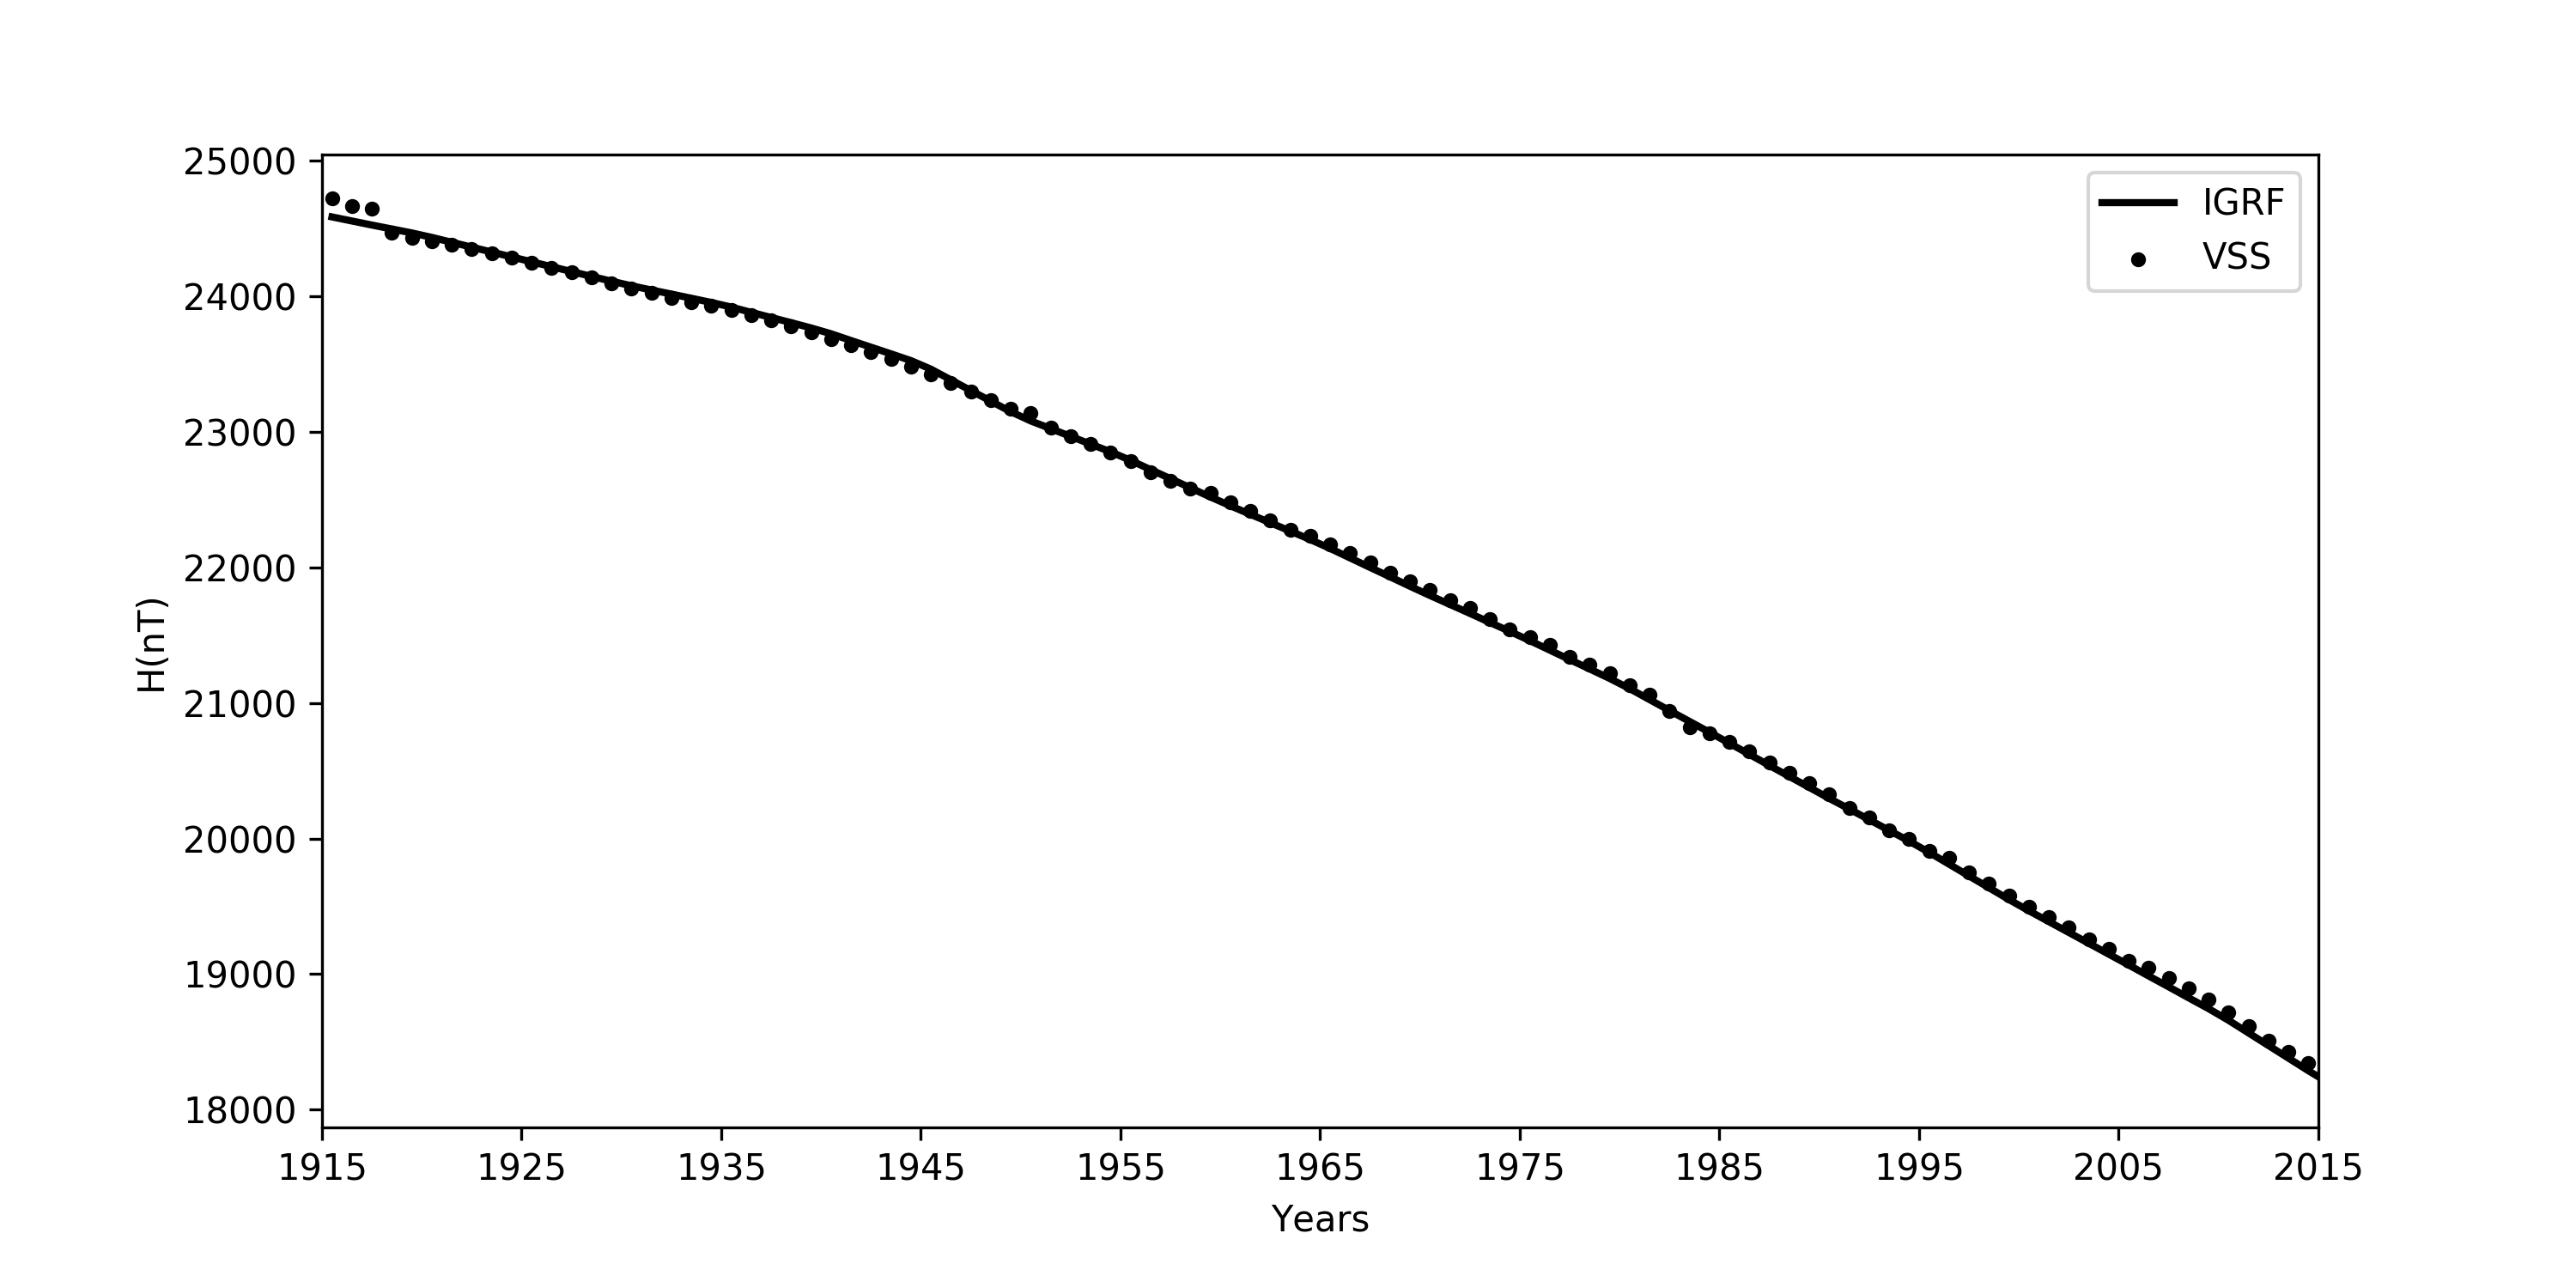
\includegraphics[width=1.0\linewidth]{H}
			\caption{2. Resultados das inversões SVD pra os modelos sintéticos I e II.}
			\label{fig:g_Sintetico}
		\end{figure}
	
\end{block}

\begin{block}{Geomagnetics Jerks}
	\justifying
	
\begin{figure}
	\centering
	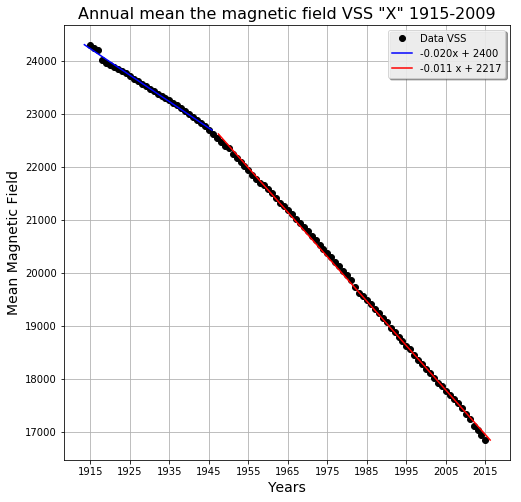
\includegraphics[width=0.6\linewidth]{retasX}
	\caption{2. Resultados das inversões SVD pra os modelos sintéticos I e II.}
	\label{fig:g_Sintetico}
\end{figure}	

	
\begin{figure}
	\centering
	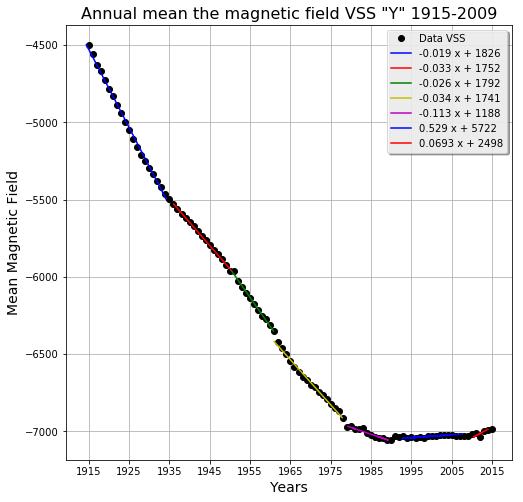
\includegraphics[width=0.6\linewidth]{retasY}
	\caption{2. Resultados das inversões SVD pra os modelos sintéticos I e II.}
	\label{fig:g_Sintetico}
\end{figure}	
	
	

	
\end{block}


%\begin{block}{Área de Estudos}
%	\justifying
%	O Campo de Pineview Figura \ref{fig:areapineview}, localizado no estado de Utah, EUA.
%	\begin{figure}[h]
%		\centering
%		\includegraphics[width=0.5\linewidth]{areapineview}
%		\caption{Mapa com a localização do Campo de Pineview, Utah, EUA. (Chidsey and Sprinkel, 2005)}
%		\label{fig:areapineview}
%	\end{figure}
	
%\end{block}
\end {column}	

%%%%%%%%%%%%%%%%%%%%%%%%%%%%%%%%%%%%%%%%%%%%%%%%%%%%%%%%%%%%%%%%%%%%%%%%%%%%%%%%%%%%%%%%%%%%%%%%%%%%%%%%%%%%
%%%%%%%%%%%%			Terceira Coluna %%%%%%%%%%%%%%%%%%%%%%%%%%%%%%%%%%%%%%%%%%%%%%%%%%%%%%%%%%%%%%%%%%%% %%%%%%%%%%%%							%%%%%%%%%%%%%%%%%%%%%%%%%%%%%%%%%%%%%%%%%%%%%%%%%%%%%%%%%%%%%%%%%%%%
%%%%%%%%%%%%%%%%%%%%%%%%%%%%%%%%%%%%%%%%%%%%%%%%%%%%%%%%%%%%%%%%%%%%%%%%%%%%%%%%%%%%%%%%%%%%%%%%%%%%%%%%%%%%
\begin{column}{.31\linewidth}


\begin{block}{}
\begin{figure}
	\centering
	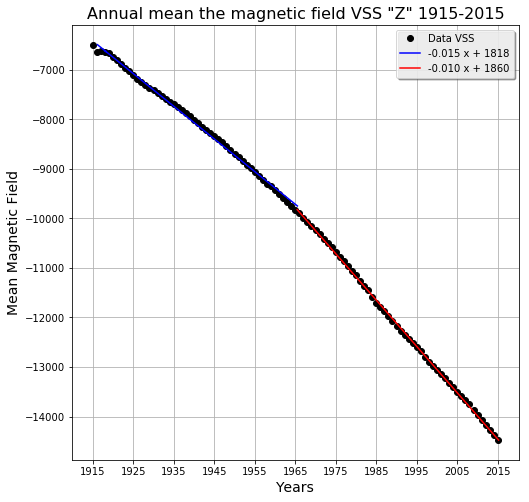
\includegraphics[width=0.6\linewidth]{retasZ}
	\caption{2. Resultados das inversões SVD pra os modelos sintéticos I e II.}
	\label{fig:g_Sintetico}
\end{figure}

	\begin{figure}
		\centering
		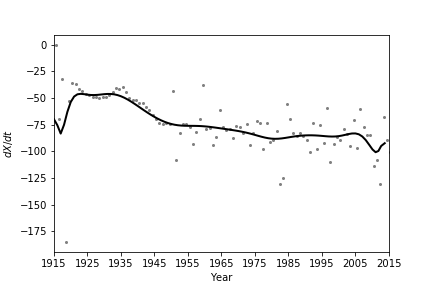
\includegraphics[width=0.7\linewidth]{spline101sv_X_spline}
		\caption{6. Estimativas dos gradientes das formações de Pineview com o método SVD para as matrizes $Z$ e $(Z{T}Z+e^{2}I)$ realizadas neste trabalho e as estimativas de gradientes com o inversão utilizando norma \textit{l1} e \textit{l2} determinadas em Deming e Chapman (1988).}
		\label{fig:g_Simposio_z1}
	\end{figure}

	\begin{figure}
\centering
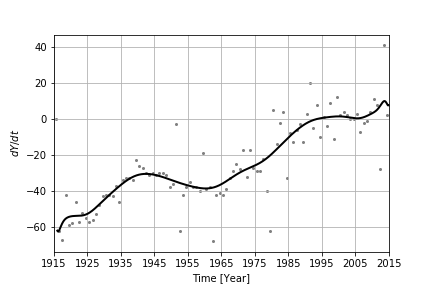
\includegraphics[width=0.7\linewidth]{spline100sv_y_spline}
\caption{6. Estimativas dos gradientes das formações de Pineview com o método SVD para as matrizes $Z$ e $(Z{T}Z+e^{2}I)$ realizadas neste trabalho e as estimativas de gradientes com o inversão utilizando norma \textit{l1} e \textit{l2} determinadas em Deming e Chapman (1988).}
\label{fig:g_Simposio_z1}
\end{figure}

\begin{figure}
\centering
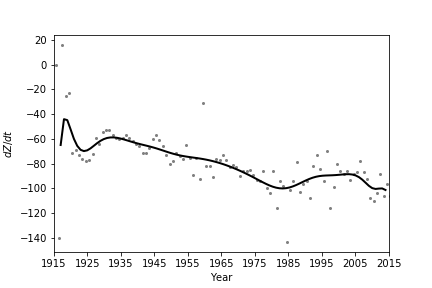
\includegraphics[width=0.7\linewidth]{spline100sv_z_spline}
\caption{7. Erro RMS entre o dado observado e calculado em relação a escolha do fator de amortecimento $e$. $e=0.5$ resulta no menor $E_{RMS}$ entre os dados.}
\label{fig:eps_erro}
\end{figure}






\end{block}


%\begin{block}{References}
%\bibliographystyle{seg} 
%\bibliography{references}
%\end{block}

\begin{block}{Conclusões}

	\begin{itemize}
\justifying	
		\item O resultado obtido na inversão apresentam valores coerentes do ponto de vista físico e semelhantes aos encontrados por Deming e Chapman (1988), na determinação dos gradientes para as formações \textbf{Tw}, \textbf{Kec} \textbf{Kk} \textbf{Jtc} e \textbf{Jn}, Figura \ref{fig:g_Simposio_z1}.
	
	\end{itemize}
	\vspace{-0.2cm}
\end{block}

\begin{block}{Referencias}

\begin{itemize}
\item Deming, D., Chapman, S. D., 1988. Inversion of Bottom-hole Temperature data: The Pineview field, Utah-Wyoming thrust belt. Geophysics, 53: 707-720.
\item Lachenbruch, A. H., Brewer, M. C., 1959, Dissipation of the temperature effect of drilling a well in Arctic Alaska. U. S. Geol. Survey Bull., 1083-C: 73-109.
\end{itemize}
\vspace{-0.2cm}
\end{block}

\end{column}

\end{columns}
\end{document}



